
\subsection{Lógica Difusa}

\subsubsection{Introducción}

A lo largo de los años hubo una gran cantidad de cambios en los paradigmas en las ciencias y matemáticas, en este caso me enfoco en el concepto de incertidumbre. Según la visión tradicional, la incertidumbre no era parte de la ciencia y esta se esforzaba en eliminarla. Según la visión alternativa, la incertidumbre juega un rol muy importante en la ciencia. \par
La lógica difusa fue investigada por primera vez por el ingeniero Lotfy A. Zadeh, en la Universidad de Berkeley (California) cuando logro comprender lo que el llamo principio de incompatibilidad: "A medida que aumenta la complejidad, las declaraciones precisas pierden significado y las declaraciones significativas pierden precisión". Lo que quiere decir es que cuando un sistema se vuelve mas complejo, nuestra capacidad de ser precisos disminuye (inherentemente debido a que la capacidad de la computación de datos no es infinita) mucho mas allá del cual la precisión y el significado son características indispensables.\par
La lógica difusa permite tomar decisiones mas o menos intensas en función de grados intermedios de cumplimiento de una premisa. Esta nueva lógica permite comprender nuestras expresiones del tipo <<hace mucho frió>>, <<él es un poco alto>>, <<su ritmo es algo lento>>, entre otras.\par
Este es uno de los temas que siempre aparece en cualquier documento, libro, artículos y/o revistas dedicada a los sistemas de control y se caracteriza por ser un sistema de control sencillo, robusto, económico, de muy rápida implementación y con la ventaja de que permite agregar múltiples entradas sin complejizar demasiado su resolución.\par

\subsubsection{Conjuntos difusos y funciones características}

Lotfy A. Zadeh utilizo el ejemplo de los hombres altos para poder explicar el concepto de conjunto difuso. Según la teoría clásica los hombres que superen cierta altura pertenecen al conjunto de hombres "altos". Así por ejemplo, tendríamos que cualquier hombre que supere 1,7 mts es considerado alto, en cambio quien pida 1,69 mts deja de considerado alto lo cual no tiene mucho sentido que un hombre sea considerado mientras que otro no cuando su altura difiere 1 cm. La lógica difusa propone un conjunto que no tiene una frontera clara, y asigna un cierto grado de pertenencia a ese conjunto, entre 0 y 1. Ejemplo: Un hombre que mida 1,49 mts tiene un grado de pertenencia del 0.8 al conjunto de hombres bajos, mientras que un hombre que mida 1.6 mts tiene un grado de pertenencia del 0.5 a este mismo conjunto.\par

\begin{center}
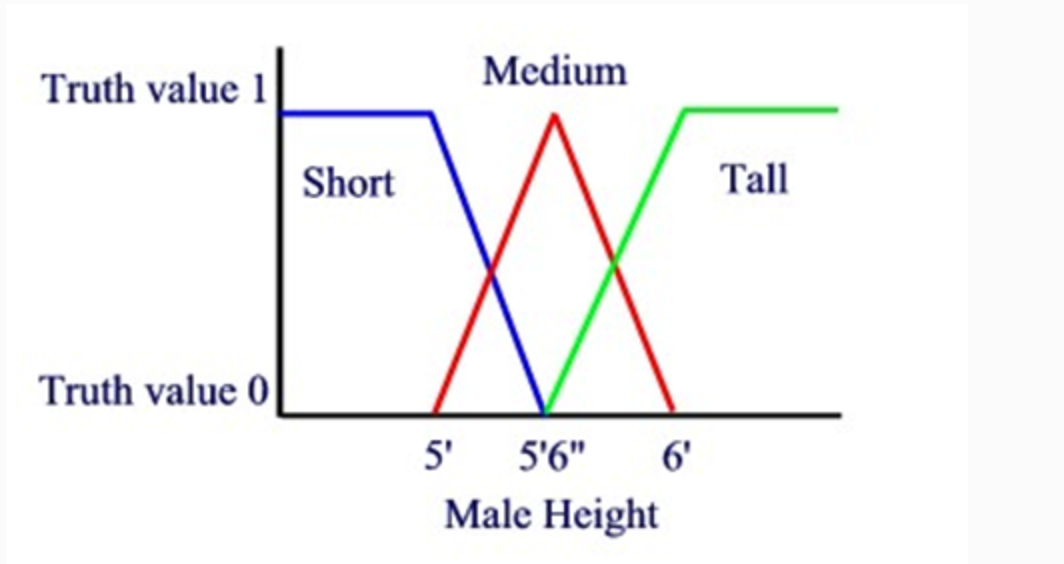
\includegraphics[scale=0.2]{Tesis/Capitulos/02_MARCO_TEORICO/img/ConjDifuso.png}
\captionof{figure}{Conjuntos difusos y funciones características}
\end{center}

Este grado de pertenencia de la persona en el conjunto se define mediante la función característica asociada al conjunto difuso. La función característica utilizada, depende del criterio que utilicemos para resolver nuestro problema. La única condición que debe cumplir una función característica es que tome valores entre 0 y 1 y sea continua.\par

Funciones características mas utilizadas: Gaussiana, Sigmoidal, Gamma, Pi, Campana, Trapezoidal, Triangular.\par

\begin{figure}[H]
    \centering
    \subfigure[]{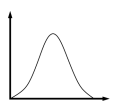
\includegraphics[width=0.2\textwidth]{Tesis/Capitulos/02_MARCO_TEORICO/img/gaussiana.png}} 
    \subfigure[]{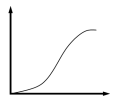
\includegraphics[width=0.2\textwidth]{Tesis/Capitulos/02_MARCO_TEORICO/img/logaritmica.png}} 
    \subfigure[]{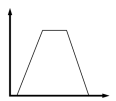
\includegraphics[width=0.2\textwidth]{Tesis/Capitulos/02_MARCO_TEORICO/img/trapezoidal.png}}
    \subfigure[]{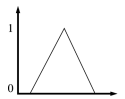
\includegraphics[width=0.2\textwidth]{Tesis/Capitulos/02_MARCO_TEORICO/img/triangular.png}}
    \caption{(a) Gaussiana (b) Sigmoidal (c) Rectangular (d) Triangular}
    \label{fig:foobar}
\end{figure}


\paragraph{Operaciones con conjuntos difusos}

\begin{itemize}
    \item Intersección:  \hfill 
    \begin{center}
        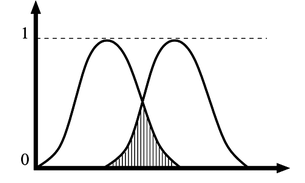
\includegraphics[scale=0.6]{Tesis/Capitulos/02_MARCO_TEORICO/img/interseccion.png}
        \captionof{figure}{Intersección }
    \end{center}
    \begin{equation}
    \tcboxmath[colback=white!25!white,colframe=black]
    {\mu( A \cap B ) (x) = min (\mu_A (x), \mu_B (x) )}  
    \end{equation}
    
    \item Unión:  \hfill 
    \begin{center}
        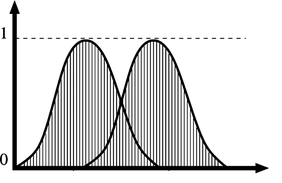
\includegraphics[scale=0.6]{Tesis/Capitulos/02_MARCO_TEORICO/img/union.png}
        \captionof{figure}{Unión }
    \end{center}
    \begin{equation}
    \tcboxmath[colback=white!25!white,colframe=black]
    {\mu( A \cup B ) (x) = max (\mu_A (x), \mu_B (x) )}  
    \end{equation}
    
    \item Complemento:  \hfill 
    \begin{center}
        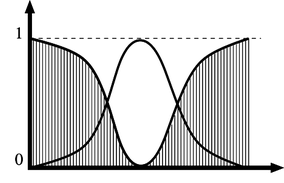
\includegraphics[scale=0.6]{Tesis/Capitulos/02_MARCO_TEORICO/img/complemento.png}
        \captionof{figure}{Complemento }
    \end{center}
    \begin{equation}
    \tcboxmath[colback=white!25!white,colframe=black]
    {\mu_A (x) = 1 - \mu_A (x)}  
    \end{equation}
    
    \item Inclusión:  \hfill  
    Un conjunto difuso, A, esta incluido en otro, B, si su función de pertenencia toma valores mas pequeños: 
    \begin{equation}
    \tcboxmath[colback=white!25!white,colframe=black]
    {\mu_B (x) \leq \mu_A (x)}  
    \end{equation}
    
\end{itemize}


\subsubsection{Reglas}

Se llama reglas difusas al conjunto de proposiciones IF-THEN que modelan el problema que uno planea resolver. Típicamente tienen la forma: \par
\bigbreak
    "Si v es A entonces c es B"
\bigbreak
Donde A y B son conjuntos difusos en los rangos de "v" y "c" respectivamente.
\bigbreak

El conjunto de reglas se definen en lenguaje natural, según el grado de pertenencia de sus variables será el grado de verdad de la regla. El comportamiento de la salida dependerá de las reglas con mayor grado de verdad.\par

\subsubsection{Control Difuso}

\begin{center}
    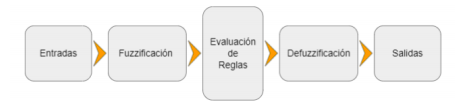
\includegraphics[scale=0.7]{Tesis/Capitulos/02_MARCO_TEORICO/img/etapas.png}
    \captionof{figure}{Proceso de control difuso}
\end{center}

Se puede descomponer el proceso de control difuso en tres etapas principales.\par

\paragraph{Fuzzificación} 

Primera parte del proceso, dados los valores de entrada se calcula el grado de pertenencia a cada uno de los conjuntos difusos considerados, mediante las funciones características asociadas a estos conjuntos difusos.\par

Por ejemplo, tomando la variable velocidad.\par

\begin{center}
    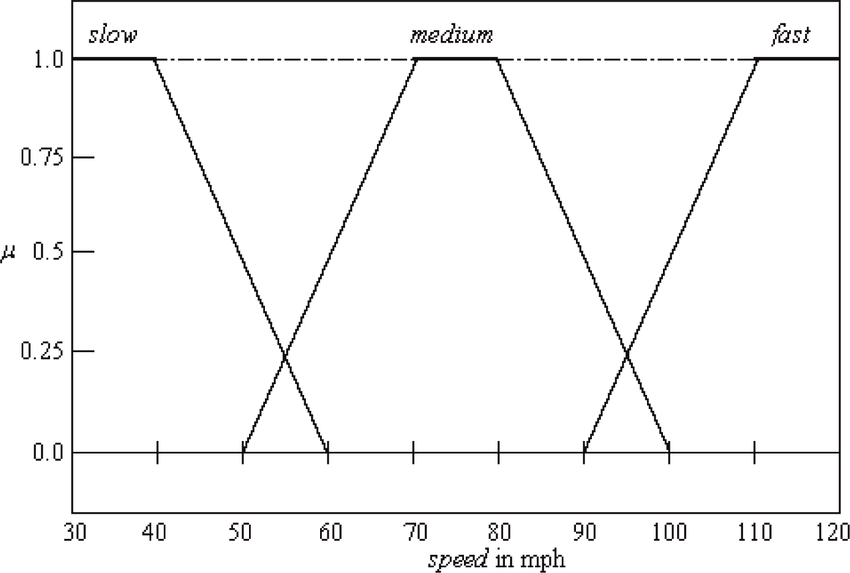
\includegraphics[scale=0.25]{Tesis/Capitulos/02_MARCO_TEORICO/img/speed.png}
    \captionof{figure}{Ejemplo Fuzzificación}
\end{center}

Con un valor de 65 mph, se cuantifica su grado de pertenencia a los conjuntos representados por algunas etiquetas lingüísticas: baja, media, alta. Para ellos se debió haber definido previamente una función de pertenencia para cada una de esas etiquetas que define que valores de la variable velocidad le pertenece y con que grado de pertenencia a cada una de ellas. Siguiendo con nuestro ejemplo, tiene un grado de pertenencia del 0 en la etiqueta ''baja''. Un grado de pertenencia del 0.75 en la etiqueta ''media'' y un 0 en la etiqueta ''alta''.\par

\paragraph{Evaluación de reglas}

Las reglas relacionan los conjuntos difusos de entrada mediante mecanismos de inferencia (reglas) con las salidas difusas.\par

Una vez terminada la etapa previa, la fuzzificación, se procede a evaluar los antecedentes de las reglas, obteniendo el grado de verdad o ''peso'' para cada una de ellas.\par

El peso de la regla estará dado por la veracidad del antecedente. Por ejemplo, si tiene una regla del tipo: \par

\begin{center}
\uline{\bfseries SI} la velocidad es ''baja'' \uline{\bfseries ENTONCES} ''aumente'' la potencia del motor.
\end{center}

Se asigna como peso el grado de pertenencia del valor leído de velocidad a la etiqueta lingüística "baja".

En el caso de que tenga una regla con conectivos lógicos \uline{\bfseries Y}:

\begin{center}
\uline{\bfseries SI} la velocidad es ''baja'' \uline{\bfseries Y} los obstáculos están ''lejos'' \uline{\bfseries ENTONCES} ''aumente'' la potencia del motor.
\end{center}

La regla sera tan verdadera como lo sea el menos verdadero de sus antecedentes. Por ende, se le asigna a la regla como peso, el menor de los grados de pertenencia de las variables de los antecedentes a las respectivas etiquetas lingüísticas.\par
Esto se repite para el resto de las reglas, entonces cada regla queda con su peso correspondiente.\par
\bigbreak
Así como cada entrada tiene sus propias funciones de pertenencia, cada salida le corresponde su propio set de funciones de pertenencia. Cada una de ella es una salida difusa (''baje'', ''no modifique'', ''aumente'' la potencia del motor).\par
\bigbreak
A cada una de las salidas difusas se les asigna un valor (grado de aplicabilidad) es el valor máximo de cada uno de los pesos de las reglas que la mencionan. De esta manera, tenemos casa salida difusa con su valor.

\paragraph{Defuzzificación}

De la etapa anterior del proceso tenemos varias salidas difusas (''baje'', ''no modifique'', ''aumente'') cada una de ellas con un valor de verdad o de aplicabilidad (un numero de 0 a 1) para cada variable de salida del sistema (en este caso la potencia del motor).\par
\bigbreak
Ahora la pregunta es, cual es la potencia del motor? Una forma fácil y efectiva de determinarlo es realizando la operación denominada C.O.G (Centro de gravedad en ingles) el cual consiste en: \par

\begin{center}
\begin{equation}
        \tcboxmath[colback=white!25!white,colframe=black]
        { u = \frac{ \int_{}^{} u. \mu(u) \cdot du }{ \int_{}^{} \mu(u) \cdot du } }  
\end{equation}
\end{center}

Ejemplo del método "Centro de gravedad" \par

\begin{center}
    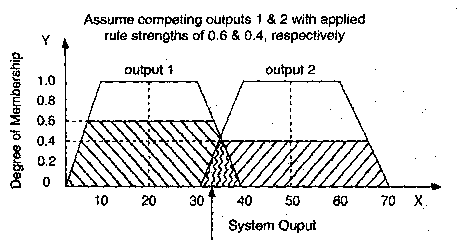
\includegraphics[scale=0.7]{Tesis/Capitulos/02_MARCO_TEORICO/img/COG.png}
    \captionof{figure}{Ejemplo C.O.G}
\end{center}

\underline{\textbf{Método del Centro de gravedad (C.O.G)}} (asumiendo que los pesos de las reglas 1 y 2 son 0.6 y 0.4 respectivamente)

\begin{itemize}
    \item Se determina el centroide de la función de pertenencia de salida. En este caso seria X=20 para la salida 1 y X=50 para la salida 2.
    \item Las funciones de pertenencia están limitadas en altura por el peso de la regla aplicada, y se calculan las áreas de las funciones de pertenencias (Área del trapecio $A=\frac{B+b}{2}.h$ ).\par
    Área de la salida 1: $A_1 =\frac{40+28}{2}.0.6 = 20.4 $ \par
    Área de la salida 2: $A_2 =\frac{40+32}{2}.0.4 = 14.4 $ \par
    \item Finalmente la salida defuzzificada es el promedio ponderado de los centroides y las áreas calculadas: Peso promedio: $W_{av} =\frac{20*20.4+14.4*50}{20.4+14.4} = 32.4 $
\end{itemize}

\underline{\textbf{Utilizando Singletons}} (asumiendo que los pesos de las reglas 1 y 2 son 0.6 y 0.4 respectivamente)

Con el propósito de simplificar el proceso de defuzzificación se utiliza un Singleton (una función de pertenencia de salida representada por una única linea vertical). De esta forma el calculo del centro de gravedad se traduce en un único calculo promedio ponderado entre los centroides y la aplicabilidad de las reglas: $W_{av} =\frac{20*0.6+50*0.4}{0.6+0.4} = 32.0 $